% 2-14-b-tree.tex

%%%%%%%%%%%%%%%%%%%%
\documentclass[a4paper, justified]{tufte-handout}

% hw-preamble.tex

% geometry for A4 paper
% See https://tex.stackexchange.com/a/119912/23098
\geometry{
  left=20.0mm,
  top=20.0mm,
  bottom=20.0mm,
  textwidth=130mm, % main text block
  marginparsep=5.0mm, % gutter between main text block and margin notes
  marginparwidth=50.0mm % width of margin notes
}

% for colors
\usepackage{xcolor} % usage: \color{red}{text}
% predefined colors
\newcommand{\red}[1]{\textcolor{red}{#1}} % usage: \red{text}
\newcommand{\blue}[1]{\textcolor{blue}{#1}}
\newcommand{\teal}[1]{\textcolor{teal}{#1}}

\usepackage{todonotes}

% heading
\usepackage{sectsty}
\setcounter{secnumdepth}{2}
\allsectionsfont{\centering\huge\rmfamily}

% for Chinese
\usepackage{xeCJK}
\usepackage{zhnumber}
\setCJKmainfont[BoldFont=FandolSong-Bold.otf]{FandolSong-Regular.otf}

% for fonts
\usepackage{fontspec}
\newcommand{\song}{\CJKfamily{song}} 
\newcommand{\kai}{\CJKfamily{kai}} 

% To fix the ``MakeTextLowerCase'' bug:
% See https://github.com/Tufte-LaTeX/tufte-latex/issues/64#issuecomment-78572017
% Set up the spacing using fontspec features
\renewcommand\allcapsspacing[1]{{\addfontfeature{LetterSpace=15}#1}}
\renewcommand\smallcapsspacing[1]{{\addfontfeature{LetterSpace=10}#1}}

% for url
\usepackage{hyperref}
\hypersetup{colorlinks = true, 
  linkcolor = teal,
  urlcolor  = teal,
  citecolor = blue,
  anchorcolor = blue}

\newcommand{\me}[4]{
    \author{
      {\bfseries 姓名:}\underline{#1}\hspace{2em}
      {\bfseries 学号:}\underline{#2}\hspace{2em}\\[10pt]
      {\bfseries 评分:}\underline{#3\hspace{3em}}\hspace{2em}
      {\bfseries 评阅:}\underline{#4\hspace{3em}}
  }
}

% Please ALWAYS Keep This.
\newcommand{\noplagiarism}{
  \begin{center}
    \fbox{\begin{tabular}{@{}c@{}}
      请独立完成作业,不得抄袭。\\
      若得到他人帮助, 请致谢。\\
      若参考了其它资料,请给出引用。\\
      鼓励讨论,但需独立书写解题过程。
    \end{tabular}}
  \end{center}
}

\newcommand{\goal}[1]{
  \begin{center}{\fcolorbox{blue}{yellow!60}{\parbox{0.50\textwidth}{\large 
    \begin{itemize}
      \item 体会``思维的乐趣''
      \item 初步了解递归与数学归纳法 
      \item 初步接触算法概念与问题下界概念
    \end{itemize}}}}
  \end{center}
}

% Each hw consists of four parts:
\newcommand{\beginrequired}{\hspace{5em}\section{作业 (必做部分)}}
\newcommand{\beginoptional}{\section{作业 (选做部分)}}
\newcommand{\beginot}{\section{Open Topics}}
\newcommand{\begincorrection}{\section{订正}}
\newcommand{\beginfb}{\section{反馈}}

% for math
\usepackage{amsmath, mathtools, amsfonts, amssymb}
\newcommand{\set}[1]{\{#1\}}

% define theorem-like environments
\usepackage[amsmath, thmmarks]{ntheorem}

\theoremstyle{break}
\theorempreskip{2.0\topsep}
\theorembodyfont{\song}
\theoremseparator{}
\newtheorem{problem}{题目}[subsection]
\renewcommand{\theproblem}{\arabic{problem}}
\newtheorem{ot}{Open Topics}

\theorempreskip{3.0\topsep}
\theoremheaderfont{\kai\bfseries}
\theoremseparator{:}
\theorempostwork{\bigskip\hrule}
\newtheorem*{solution}{解答}
\theorempostwork{\bigskip\hrule}
\newtheorem*{revision}{订正}

\theoremstyle{plain}
\newtheorem*{cause}{错因分析}
\newtheorem*{remark}{注}

\theoremstyle{break}
\theorempostwork{\bigskip\hrule}
\theoremsymbol{\ensuremath{\Box}}
\newtheorem*{proof}{证明}

% \newcommand{\ot}{\blue{\bf [OT]}}

% for figs
\renewcommand\figurename{图}
\renewcommand\tablename{表}

% for fig without caption: #1: width/size; #2: fig file
\newcommand{\fig}[2]{
  \begin{figure}[htbp]
    \centering
    \includegraphics[#1]{#2}
  \end{figure}
}
% for fig with caption: #1: width/size; #2: fig file; #3: caption
\newcommand{\figcap}[3]{
  \begin{figure}[htbp]
    \centering
    \includegraphics[#1]{#2}
    \caption{#3}
  \end{figure}
}
% for fig with both caption and label: #1: width/size; #2: fig file; #3: caption; #4: label
\newcommand{\figcaplbl}[4]{
  \begin{figure}[htbp]
    \centering
    \includegraphics[#1]{#2}
    \caption{#3}
    \label{#4}
  \end{figure}
}
% for margin fig without caption: #1: width/size; #2: fig file
\newcommand{\mfig}[2]{
  \begin{marginfigure}
    \centering
    \includegraphics[#1]{#2}
  \end{marginfigure}
}
% for margin fig with caption: #1: width/size; #2: fig file; #3: caption
\newcommand{\mfigcap}[3]{
  \begin{marginfigure}
    \centering
    \includegraphics[#1]{#2}
    \caption{#3}
  \end{marginfigure}
}

\usepackage{fancyvrb}

% for algorithms
\usepackage[]{algorithm}
\usepackage[]{algpseudocode} % noend
% See [Adjust the indentation whithin the algorithmicx-package when a line is broken](https://tex.stackexchange.com/a/68540/23098)
\newcommand{\algparbox}[1]{\parbox[t]{\dimexpr\linewidth-\algorithmicindent}{#1\strut}}
\newcommand{\hStatex}[0]{\vspace{5pt}}
\makeatletter
\newlength{\trianglerightwidth}
\settowidth{\trianglerightwidth}{$\triangleright$~}
\algnewcommand{\LineComment}[1]{\Statex \hskip\ALG@thistlm \(\triangleright\) #1}
\algnewcommand{\LineCommentCont}[1]{\Statex \hskip\ALG@thistlm%
  \parbox[t]{\dimexpr\linewidth-\ALG@thistlm}{\hangindent=\trianglerightwidth \hangafter=1 \strut$\triangleright$ #1\strut}}
\makeatother

% for footnote/marginnote
% see https://tex.stackexchange.com/a/133265/23098
\usepackage{tikz}
\newcommand{\circled}[1]{%
  \tikz[baseline=(char.base)]
  \node [draw, circle, inner sep = 0.5pt, font = \tiny, minimum size = 8pt] (char) {#1};
}
\renewcommand\thefootnote{\protect\circled{\arabic{footnote}}} % feel free to modify this file
%%%%%%%%%%%%%%%%%%%%
\title{第14讲: B 树}
\me{林凡琪 }{211240042}{}{}
\date{\zhtoday} % or like 2019年9月13日
%%%%%%%%%%%%%%%%%%%%
\begin{document}
\maketitle
%%%%%%%%%%%%%%%%%%%%
\noplagiarism % always keep this line
%%%%%%%%%%%%%%%%%%%%
\begin{abstract}
  % \begin{center}{\fcolorbox{blue}{yellow!60}{\parbox{0.65\textwidth}{\large 
  %   \begin{itemize}
  %     \item 
  %   \end{itemize}}}}
  % \end{center}
\end{abstract}
%%%%%%%%%%%%%%%%%%%%
\beginrequired

%%%%%%%%%%%%%%%
\begin{problem}[TC 18.1-1]
\end{problem}

\begin{solution}
  根据定义,最小度 tt 意味着除根以外的每个节点都必须至少有 t - 1 个key,因此除根以外的每个内部节点都至少有 tt 个子节点。 因此,当 t = 1 时,意味着除根之外的每个节点都必须至少有 t - 1 = 0 个key,因此除根之外的每个内部节点都至少有 t = 1 个子节点。\\
  因此,我们可以看到最小情况不存在,因为在 B 树中不存在具有 0 个key的节点,并且不存在只有 1 个子节点的节点.
\end{solution}
%%%%%%%%%%%%%%%

%%%%%%%%%%%%%%%
\begin{problem}[TC 18.1-4]
\end{problem}

\begin{solution}
  $$
    \begin{aligned}
      n & = (1 + 2t + (2t)^2 + … + (2t)^h) * (2t - 1) \\
        & = (2t)^{h + 1} - 1
    \end{aligned}
  $$
\end{solution}
%%%%%%%%%%%%%%%

%%%%%%%%%%%%%%%
\begin{problem}[TC 18.2-3]
\end{problem}

\begin{solution}
  在 B-tree 中找到最小值与在二叉搜索树中找到最小值非常相似。 我们需要为给定的根找到最左边的叶子,并返回第一个键\\
  x 是 B-tree T 上的一个节点。顶层调用是 B-TREE-FIND-MIN(T.root)\\
  FCTVAL 是存储在以 x 为根的子树中的最小key
  \begin{algorithm}
    \begin{algorithmic}[1]
      \Procedure{b-tree-find-min}{x}
      \If{x = NIL}
      \Return NIL
      \ElsIf{x.leaf}
      \Return x.key[1]
      \Else
      \State DISK-READ(x.c[1])
      \Return B-TREE-FIND-MIN(x.c[1])
      \EndIf
      \EndProcedure
    \end{algorithmic}
  \end{algorithm}
  根据以下规则查找给定密钥 $x.key_i$ 的前继:

  如果 x 不是叶节点,则返回 x 的第 i 个子节点中的最大键,这也是以 $x.c_i$ 为根的子树的最大key

  如果 x 是叶节点并且 i > 1,则返回 x 的第 (i - 1) 个key,即 $x.key_{i - 1}$

  否则,查找最后一个节点 y(从下向上)且 j > 0,使得 $x.key_i$ 是 $y.c_j$ 中最左边的key; 如果 j = 1,则返回 $\text{NIL}$,因为 $x.key_i$x.key 是树中的最小key; 否则我们返回 $y.key_{j - 1}$

  x 是 B 树 T 上的一个节点。 i 是键的索引。

  FCTVAL 是 $x.key_i$ 的前身

  \begin{algorithm}
    \begin{algorithmic}[2]
      \Procedure{b-tree-predecessor}{x, i}
      \If{!x.leaf}
      \State DISK-READ(x.c[i])
      \Return B-TREE-FIND-MAX(x.c[i])
      \ElsIf{i > 1}
      \Return x.key[i - 1]
      \Else
      \State z$\gets$x
      \While{true}
      \If{z.p = NIL}
      \Return NIL
      \EndIf
      \State y$\gets$z.p
      \State j$\gets$1
      \State DISK-READ(y.c[1])
      \While{y.c[j] != x}
      \State j$\gets$j + 1
      \State DISK-READ(y.c[j])
      \EndWhile
      \If{j = 1}
      \State z$\gets$y
      \Else
      \Return y.key[j - 1]
      \EndIf
      \EndWhile
      \EndIf
      \EndProcedure
    \end{algorithmic}
  \end{algorithm}

  x 是 B-tree TT 上的一个节点。 顶层调用是 $\text{B-TREE-FIND-MAX}(T.root)$

  $\text{FCTVAL}$ 是存储在以 x 为根的子树中的最大key。\\
  \begin{algorithm}
    \begin{algorithmic}[3]
      \Procedure{b-tree-find-max}{x}
      \If{x = NIL}
      \Return NIL
      \ElsIf{x.leaf}
      \Return x.[x.n]
      \Else
      \State DISK-READ(x.c[x.n + 1])
      \Return B-TREE-FIND-MAX(x.c[x.n + 1])
      \EndIf
      \EndProcedure
    \end{algorithmic}
  \end{algorithm}
\end{solution}
%%%%%%%%%%%%%%%

%%%%%%%%%%%%%%%
\begin{problem}[TC 18.3-1]
\end{problem}

\begin{solution}
  \begin{figure}
    \centering
    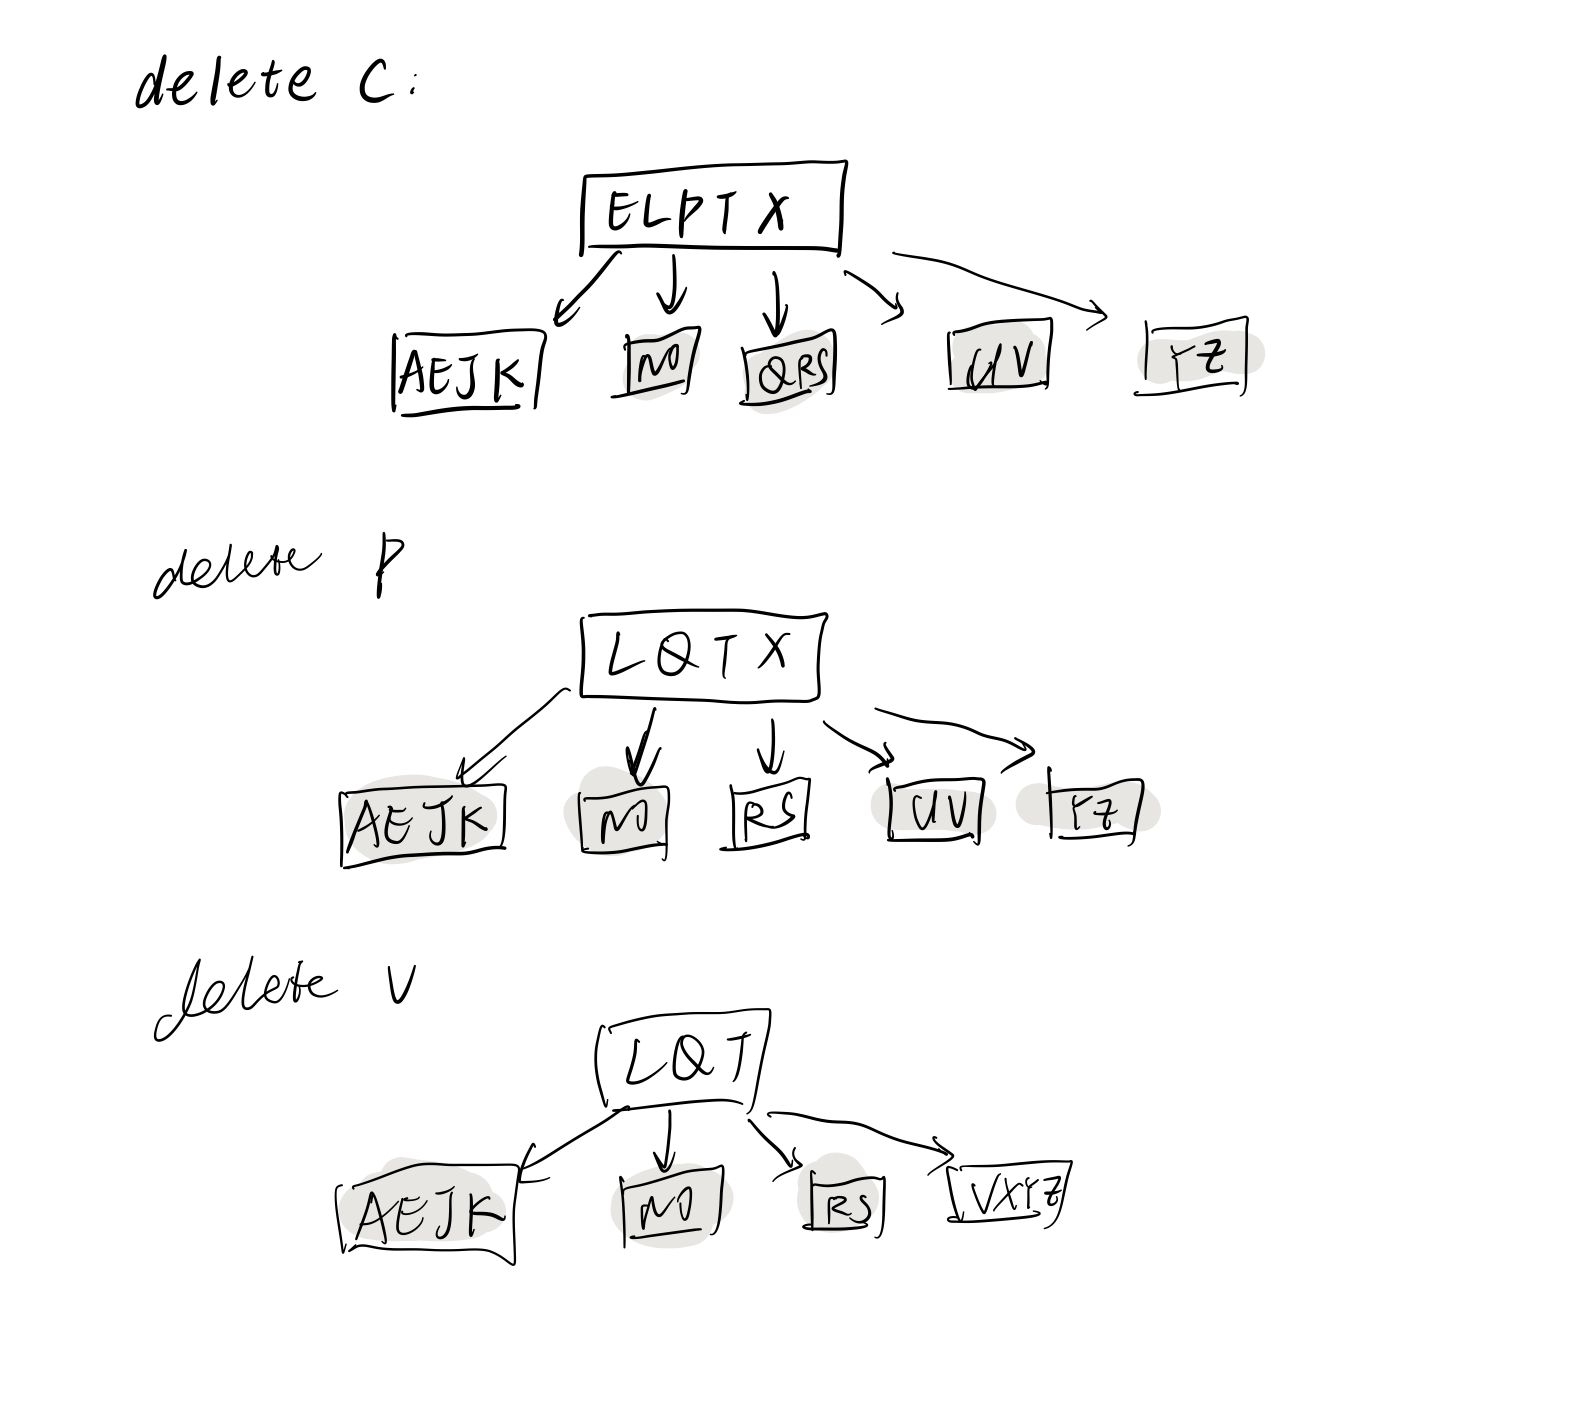
\includegraphics[width=4cm,height=5cm]{pic.jpg}
  \end{figure}
\end{solution}
%%%%%%%%%%%%%%%

%%%%%%%%%%%%%%%%%%%%
\beginoptional

%%%%%%%%%%%%%%%
\begin{problem}[TC 18.2-4\red{$^{\star}$}]
\end{problem}

\begin{solution}
\end{solution}
%%%%%%%%%%%%%%%

%%%%%%%%%%%%%%%%%%%%
\beginot

%%%%%%%%%%%%%%%
\begin{ot}[T-tree]
  介绍 T-tree (具体的rotation过程可以不用详细介绍)。

  \noindent 参考资料:
  \begin{itemize}
    \item \href{https://en.wikipedia.org/wiki/T-tree}{https://en.wikipedia.org/wiki/T-tree}
  \end{itemize}
\end{ot}
%%%%%%%%%%%%%%


\begin{ot}[R-tree]
  介绍 R-tree。

  \noindent 参考资料:
  \begin{itemize}
    \item \href{https://en.wikipedia.org/wiki/R-tree}{https://en.wikipedia.org/wiki/R-tree}
  \end{itemize}
\end{ot}
%%%%%%%%%%%%%%
% \begin{solution}
% \end{solution}
%%%%%%%%%%%%%%%
% \vspace{0.50cm}
%%%%%%%%%%%%%%%
% \begin{ot}[]
% 
%   \noindent 参考资料:
%   \begin{itemize}
%     \item 
%   \end{itemize}
% \end{ot}

% \begin{solution}
% \end{solution}
%%%%%%%%%%%%%%%

%%%%%%%%%%%%%%%%%%%%
% 如果没有需要订正的题目,可以把这部分删掉

% \begincorrection
%%%%%%%%%%%%%%%%%%%%

%%%%%%%%%%%%%%%%%%%%
% 如果没有反馈,可以把这部分删掉
\beginfb

% 你可以写
% ~\footnote{优先推荐 \href{problemoverflow.top}{ProblemOverflow}}:
% \begin{itemize}
%   \item 对课程及教师的建议与意见
%   \item 教材中不理解的内容
%   \item 希望深入了解的内容
%   \item $\cdots$
% \end{itemize}
%%%%%%%%%%%%%%%%%%%%
% \bibliography{2-5-solving-recurrence}
% \bibliographystyle{plainnat}
%%%%%%%%%%%%%%%%%%%%
\end{document}